\section{Implementasi Fitur Utama}
\subsection{Upload dan Pratinjau PDF}
Pengguna dapat mengunggah file PDF yang akan disimpan pada \texttt{Vercel Blob}. File ini kemudian dimuat dan dipratinjau menggunakan \texttt{PDF.js}.
\begin{lstlisting}[language=TypeScript, caption={Chat dengan AI}]
import { put } from '@vercel/blob';
import { NextResponse } from 'next/server';
import { z } from 'zod';

import { auth } from '@/app/(auth)/auth';

// Use Blob instead of File since File is not available in Node.js environment
const FileSchema = z.object({
  file: z
    .instanceof(Blob)
    .refine((file) => file.size <= 5 * 1024 * 1024, {
      message: 'File size should be less than 5MB',
    })
    // Update the file type based on the kind of files you want to accept
    .refine(
      (file) =>
        ['image/jpeg', 'image/png', 'application/pdf'].includes(file.type),
      {
        message: 'File type should be JPEG or PNG or PDF',
      },
    ),
});

export async function POST(request: Request) {
  const session = await auth();

  if (!session) {
    return NextResponse.json({ error: 'Unauthorized' }, { status: 401 });
  }

  if (request.body === null) {
    return new Response('Request body is empty', { status: 400 });
  }

  try {
    const formData = await request.formData();
    const file = formData.get('file') as Blob;

    if (!file) {
      return NextResponse.json({ error: 'No file uploaded' }, { status: 400 });
    }

    const validatedFile = FileSchema.safeParse({ file });

    if (!validatedFile.success) {
      const errorMessage = validatedFile.error.errors
        .map((error) => error.message)
        .join(', ');

      return NextResponse.json({ error: errorMessage }, { status: 400 });
    }

    // Get filename from formData since Blob doesn't have name property
    const filename = (formData.get('file') as File).name;
    const fileBuffer = await file.arrayBuffer();

    try {
      const data = await put(`${filename}`, fileBuffer, {
        access: 'public',
      });

      return NextResponse.json(data);
    } catch (error) {
      return NextResponse.json({ error: 'Upload failed' }, { status: 500 });
    }
  } catch (error) {
    return NextResponse.json(
      { error: 'Failed to process request' },
      { status: 500 },
    );
  }
}
\end{lstlisting}
Cuplikan kode pada Listing~\ref{lst:pdf-anotasi} menunjukkan bagaimana sistem menampilkan pratinjau dokumen PDF beserta fitur anotasi dalam antarmuka pengguna. Komponen ini dibungkus dalam komponen kondisional \texttt{<Show>} yang hanya akan menampilkan pratinjau jika beberapa kondisi terpenuhi: nilai \texttt{attachmentUrl} tidak kosong, \texttt{isPdfVisible} bernilai \texttt{true}, dan aplikasi tidak sedang diakses melalui perangkat seluler (\texttt{!isMobile}).
\singlespacing{}
Di dalam elemen \texttt{<div>}, komponen \texttt{<PDFViewer>} dipanggil dengan dua properti, yaitu \texttt{chatId} dan \texttt{url}. Properti \texttt{chatId} digunakan untuk mengidentifikasi percakapan yang sedang berlangsung, sementara \texttt{url} merupakan alamat file PDF yang diunggah oleh pengguna dan akan ditampilkan. Komponen \texttt{PDFViewer} ini bertanggung jawab untuk menampilkan isi dokumen PDF, serta mendukung anotasi seperti penandaan teks (highlight), penambahan catatan, atau interaksi pengguna lainnya secara langsung di dalam file.
\singlespacing{}
Implementasi pratinjau PDF ini memanfaatkan pustaka \texttt{PDF.js} dari Mozilla untuk merender halaman PDF ke dalam elemen HTML dan menangani interaksi pengguna. Tampilan dibuat responsif dan ramah pengguna, dengan \texttt{overflow-y-auto} yang memungkinkan pengguna menggulir dokumen secara vertikal. Penggunaan \texttt{Tailwind CSS} dalam kelas-kelas seperti \texttt{flex-1}, \texttt{md:w-1/2}, dan \texttt{bg-gray-100} memastikan layout antarmuka tetap estetis dan fungsional.
\singlespacing{}
\begin{lstlisting}[language=TypeScript, caption={Pratinjau \textit{PDF} dengan fitur anotasi}, label={lst:pdf-anotasi}]
<Show
  when={
    Boolean(attachmentUrl) &&
    attachmentUrl !== '' &&
    isPdfVisible &&
    !isMobile
  }
>
  <div className="flex-1 md:w-1/2 overflow-y-auto bg-gray-100">
    <PDFViewer chatId={id} url={attachmentUrl as string} />
  </div>
</Show>
\end{lstlisting}

\subsection{Tanya Jawab Berbasis RAG}
Sistem menggunakan pipeline \texttt{Langchain} untuk menjalankan \textit{Retrieval-Augmented Generation}:
\begin{enumerate}
  \item Ekstraksi teks dari PDF
  \item Pemecahan menjadi chunk dengan overlap
  \item Embedding menggunakan model dari \texttt{OpenAI API}
  \item Penyimpanan dalam vektor menggunakan \texttt{ChromaDB}
  \item Retrieval saat tanya jawab berdasarkan \texttt{cosine similarity}
  \item Prompt otomatis digabung dengan hasil retrieval dan dikirim ke model GPT
\end{enumerate}
\begin{lstlisting}[language=TypeScript, caption={Chat dengan AI}]
'use client';

import { ChatHeader } from '@/components/chat-header';
import { useArtifactSelector } from '@/hooks/use-artifact';
import type { Vote } from '@/lib/db/schema';
import { fetcher, generateUUID } from '@/lib/utils';
import { useChat } from '@ai-sdk/react';
import type { Attachment, UIMessage } from 'ai';
import type { Session } from 'next-auth';
import { useRouter, useSearchParams } from 'next/navigation';
import { useEffect, useRef, useState } from 'react';
import useSWR, { useSWRConfig } from 'swr';
import { unstable_serialize } from 'swr/infinite';
import { Artifact } from './artifact';
import { Messages } from './messages';
import { MultimodalInput } from './multimodal-input';
import { getChatHistoryPaginationKey } from './sidebar-history';
import { toast } from './toast';
import type { VisibilityType } from './visibility-selector';

import dynamic from 'next/dynamic';
const PDFViewer = dynamic(() => import('../components/pdf-viewer'), {
  ssr: false,
});

import { Show } from './shared/show';
import { useBoolean } from '@/hooks/use-boolean';
import { useMediaQuery } from 'usehooks-ts';

export function Chat({
  id,
  initialMessages,
  selectedChatModel,
  selectedVisibilityType,
  isReadonly,
  session,
  attachmentUrl,
}: {
  id: string;
  initialMessages: Array<UIMessage>;
  selectedChatModel: string;
  selectedVisibilityType: VisibilityType;
  isReadonly: boolean;
  session: Session;
  attachmentUrl?: string;
}) {
  const { mutate } = useSWRConfig();
  const isPDFSubmitted = useRef(false);
  const router = useRouter();

  const {
    messages,
    setMessages,
    handleSubmit,
    input,
    setInput,
    append,
    status,
    stop,
    reload,
  } = useChat({
    id,
    initialMessages,
    experimental_throttle: 100,
    sendExtraMessageFields: true,
    generateId: generateUUID,
    experimental_prepareRequestBody: (body) => ({
      id,
      message: body.messages.at(-1),
      selectedChatModel,
    }),
    onFinish: () => {
      mutate(unstable_serialize(getChatHistoryPaginationKey));
    },
    onResponse: () => {
      if (isPDFSubmitted.current) return;
      isPDFSubmitted.current = true;
      router.refresh();
      return;
    },
    onError: (error) => {
      toast({
        type: 'error',
        description: error.message,
      });
    },
  });

  const searchParams = useSearchParams();
  const query = searchParams.get('query');

  const [hasAppendedQuery, setHasAppendedQuery] = useState(false);

  useEffect(() => {
    if (query && !hasAppendedQuery) {
      append({
        role: 'user',
        content: query,
      });

      setHasAppendedQuery(true);
      window.history.replaceState({}, '', `/chat/${id}`);
    }
  }, [query, append, hasAppendedQuery, id]);

  const { data: votes } = useSWR<Array<Vote>>(
    messages.length >= 2 ? `/api/vote?chatId=${id}` : null,
    fetcher,
  );

  const [attachments, setAttachments] = useState<Array<Attachment>>([]);
  const { value: isPdfVisible, toggle: togglePdfVisible } = useBoolean(true);
  const isArtifactVisible = useArtifactSelector((state) => state.isVisible);
  const isMobile = useMediaQuery('(max-width: 1024px)');

  return (
    <>
      <div
        className={`flex flex-col min-w-0 h-dvh bg-background ${
          attachmentUrl ? 'md:flex-row' : ''
        }`}
      >
        <div
          className={`flex flex-col flex-1 ${attachmentUrl ? 'md:w-1/2' : 'w-full'}`}
        >
          <ChatHeader
            chatId={id}
            selectedModelId={selectedChatModel}
            selectedVisibilityType={selectedVisibilityType}
            isReadonly={isReadonly}
            session={session}
            isPdfVisible={isPdfVisible}
            onPdfToggle={togglePdfVisible}
            showPdfToggle={Boolean(attachmentUrl)}
          />

          {/* mobile pdf viewer */}
          <Show
            when={
              Boolean(attachmentUrl) &&
              attachmentUrl !== '' &&
              isPdfVisible &&
              isMobile
            }
          >
            <PDFViewer chatId={id} url={attachmentUrl as string} />
          </Show>

          <Messages
            chatId={id}
            status={status}
            votes={votes}
            messages={messages}
            setMessages={setMessages}
            reload={reload}
            isReadonly={isReadonly}
            isArtifactVisible={isArtifactVisible}
          />

          <form className="flex mx-auto px-4 bg-background pb-4 md:pb-6 gap-2 w-full md:max-w-3xl">
            <Show when={!isReadonly}>
              <MultimodalInput
                chatId={id}
                input={input}
                setInput={setInput}
                handleSubmit={handleSubmit}
                status={status}
                stop={stop}
                attachments={attachments}
                setAttachments={setAttachments}
                messages={messages}
                setMessages={setMessages}
                append={append}
              />
            </Show>
          </form>
        </div>

        <Show
          when={
            Boolean(attachmentUrl) &&
            attachmentUrl !== '' &&
            isPdfVisible &&
            !isMobile
          }
        >
          <div className="flex-1 md:w-1/2 overflow-y-auto bg-gray-100">
            <PDFViewer chatId={id} url={attachmentUrl as string} />
          </div>
        </Show>
      </div>

      <Artifact
        chatId={id}
        input={input}
        setInput={setInput}
        handleSubmit={handleSubmit}
        status={status}
        stop={stop}
        attachments={attachments}
        setAttachments={setAttachments}
        append={append}
        messages={messages}
        setMessages={setMessages}
        reload={reload}
        votes={votes}
        isReadonly={isReadonly}
      />
    </>
  );
}
\end{lstlisting}

\subsection{Retrieval-Augmented Generation}
Agar LLM dapat bekerja dengan dokumen pribadi seperti PDF, konten dokumen harus diproses dan disimpan dengan cara yang dapat diakses secara efisien oleh LLM.\@ Seluruh proses ini dikenal sebagai \emph{ingestion} \citep[p~.84]{oshin2024learning}. Ide intinya adalah mengubah teks menjadi representasi numerik yang disebut \emph{embeddings} dan menyimpannya dalam penyimpanan \emph{vektor store} (sejenis basis data vektor). Hal ini memungkinkan aplikasi untuk menemukan dan mengambil bagian yang paling relevan dari dokumen untuk menjawab pertanyaan spesifik pengguna. Proses ini melibatkan empat langkah utama:
\begin{enumerate}
  \item \emph{Loading}: Mengekstrak teks dari dokumen PDF.
  \item \emph{Splitting}: Memecah teks yang diekstrak menjadi bagian yang lebih kecil dan mudah dikelola.
  \item \emph{Embedding}: Mengubah setiap potongan teks menjadi vektor numerik yang menangkap makna semantiknya.
  \item \emph{Storing}: Menyimpan \emph{embeddings} ini dalam penyimpanan vektor untuk pencarian yang efisien.
\end{enumerate}

\begin{figure}[htbp]
  \centering
  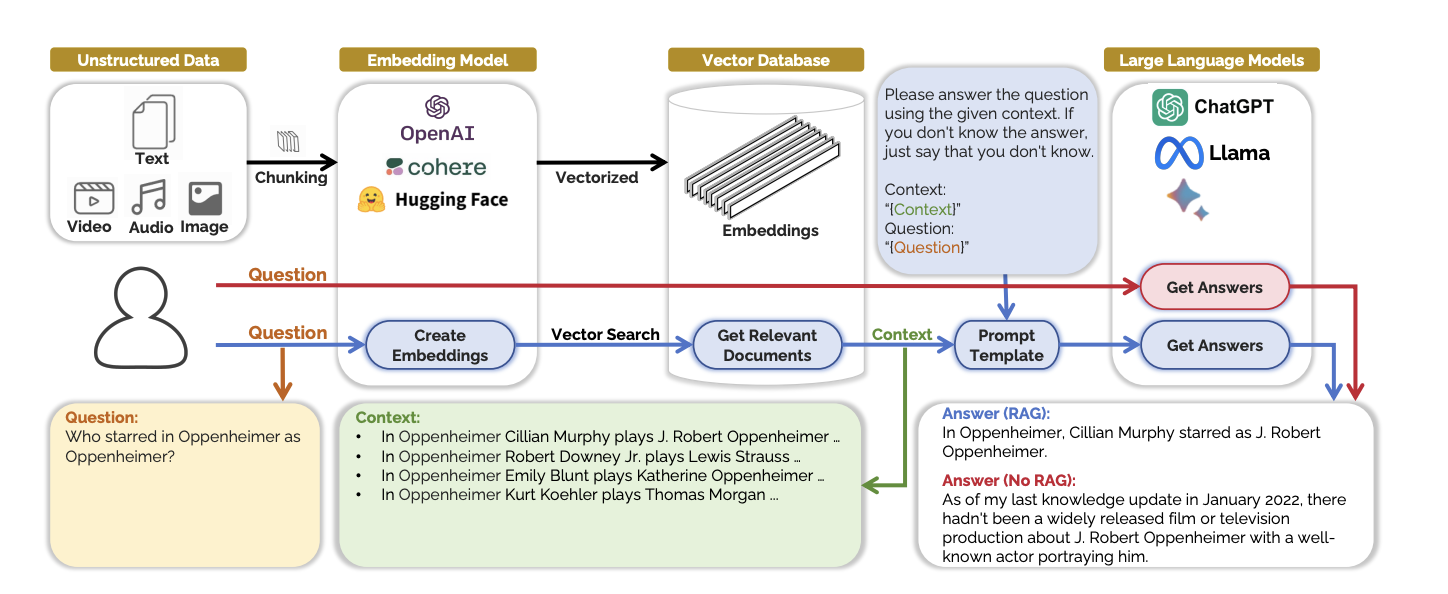
\includegraphics[width=0.85\linewidth]{images/bab-3/embeddings.png}
  \caption{Contoh \emph{RAG framework} yang menggunakan \emph{Vector Database}.}\label{fig:RAG-Framework}\citep{Jing}
\end{figure}

\subsection{Pembuatan Sitasi Otomatis}
Sistem melakukan ekstraksi metadata seperti judul, penulis, tahun, dan DOI dari PDF dan menyusunnya ke dalam format referensi (APA, MLA, IEEE, Harvard) secara otomatis.

\begin{lstlisting}[language=TypeScript, caption={Pembuatan Sitasi}, inputencoding=utf8]
'use client';
import { PaginationControls } from '@/components/citations/pagination-control';
import { Show } from '@/components/shared/show';
import { toast } from '@/components/toast';
import { Button } from '@/components/ui/button';
import {
  Card,
  CardContent,
  CardDescription,
  CardFooter,
  CardHeader,
  CardTitle,
} from '@/components/ui/card';
import { Input } from '@/components/ui/input';
import {
  Select,
  SelectContent,
  SelectItem,
  SelectTrigger,
  SelectValue,
} from '@/components/ui/select';
import { Skeleton } from '@/components/ui/skeleton';
import { citationStyles } from '@/lib/constants';
import { logger } from '@/lib/utils';
import { citationReducer, initialCitationState } from '@/reducer/citation';
import type { CitationResponse } from '@/types/citations';
import { ArrowLeft, Copy, FileText, Search } from 'lucide-react';
import Link from 'next/link';
import { useRouter, useSearchParams } from 'next/navigation';
import { useEffect, useReducer } from 'react';

const ITEMS_PER_PAGE = 10;

export default function CitationPage() {
  const searchParams = useSearchParams();
  const router = useRouter();
  const currentPage = Number(searchParams.get('page')) || 1;

  const [state, dispatch] = useReducer(citationReducer, initialCitationState);

  const setCurrentPage = (page: number) => {
    const newParams = new URLSearchParams(searchParams);
    newParams.set('page', page.toString());
    router.push(`?${newParams.toString()}`);
  };

  useEffect(() => {
    fetchCitations(currentPage);
  }, [currentPage, state.sortBy]);

  const fetchCitations = async (page: number) => {
    dispatch({ type: 'SET_LOADING_CITATIONS', payload: true });

    try {
      const response = await fetch(
        `/api/citation/save?page=${page}&limit=${ITEMS_PER_PAGE}&sortBy=${state.sortBy}`,
      );

      if (!response.ok) throw new Error('Failed to fetch citations');

      const data: CitationResponse = await response.json();
      const totalCount = data.meta?.total || 0;
      const calculatedTotalPages = Math.ceil(totalCount / ITEMS_PER_PAGE);

      dispatch({
        type: 'SET_CITATIONS_DATA',
        payload: {
          citations: data.data || [],
          totalCitations: totalCount,
          totalPages: calculatedTotalPages > 0 ? calculatedTotalPages : 1,
          hasPrev: data.meta?.has_prev_page || false,
          hasNext: data.meta?.has_next_page || false,
        },
      });
    } catch (error) {
      logger.error('failed to fetch citations:', error);
      toast({
        type: 'error',
        description: 'Failed to fetch citations',
      });
      dispatch({ type: 'RESET_CITATIONS' });
    } finally {
      dispatch({ type: 'SET_LOADING_CITATIONS', payload: false });
    }
  };

  const handleGenerateCitation = async () => {
    if (!state.doi) {
      toast({
        type: 'error',
        description: 'Please enter a DOI',
      });
      return;
    }

    dispatch({ type: 'SET_LOADING', payload: true });
    try {
      const response = await fetch('/api/citation', {
        method: 'POST',
        headers: { 'Content-Type': 'application/json' },
        body: JSON.stringify({ doi: state.doi, style: state.style }),
      });

      if (!response.ok) {
        throw new Error('Failed to generate citation');
      }

      const data = await response.json();

      dispatch({
        type: 'SET_CITATION',
        payload: data?.data,
      });

      await fetch('/api/citation/save', {
        method: 'POST',
        headers: { 'Content-Type': 'application/json' },
        body: JSON.stringify({
          doi: state.doi,
          style: state.style,
          content: data.data,
        }),
      });

      toast({
        type: 'success',
        description: 'Citation generated and saved successfully',
      });

      setCurrentPage(1);
      fetchCitations(1);
    } catch (error) {
      console.error('[ERROR]: Failed to generate citation:', error);
      toast({
        type: 'error',
        description:
          error instanceof Error
            ? error.message
            : 'Failed to generate citation',
      });
    } finally {
      dispatch({ type: 'SET_LOADING', payload: false });
    }
  };

  const handleDelete = async (id: string) => {
    try {
      const response = await fetch(`/api/citation/save/${id}`, {
        method: 'DELETE',
      });

      if (!response.ok) throw new Error('Failed to delete citation');

      toast({
        type: 'success',
        description: 'Citation deleted successfully',
      });

      fetchCitations(currentPage);
    } catch (error) {
      console.error('[ERROR]: Failed to delete citation:', error);
      toast({
        type: 'error',
        description:
          error instanceof Error ? error.message : 'Failed to delete citation',
      });
    }
  };

  const handleExport = async () => {
    try {
      const response = await fetch('/api/citation/export');
      if (!response.ok) throw new Error('Failed to export citations');

      const text = await response.text();
      const blob = new Blob([text], { type: 'text/plain' });
      const url = window.URL.createObjectURL(blob);
      const a = document.createElement('a');
      a.href = url;
      a.download = 'citations.txt';
      a.click();
      window.URL.revokeObjectURL(url);

      toast({
        type: 'success',
        description: 'Citations exported successfully',
      });
    } catch (error) {
      console.error('[ERROR]: Failed to export citations:', error);
      toast({
        type: 'error',
        description:
          error instanceof Error ? error.message : 'Failed to export citations',
      });
    }
  };

  const copyToClipboard = (text: string) => {
    if (text.length < 1) {
      toast({
        type: 'error',
        description: 'No citation to copy',
      });
      return;
    }
    navigator.clipboard.writeText(text);
    toast({
      type: 'success',
      description: 'Citations copied to clipboard',
    });
  };

  return (
    <div className="flex flex-col items-center justify-center min-h-screen bg-background p-4">
      <div className="w-full max-w-5xl">
        <div className="mb-6">
          <Link
            href="/"
            className="inline-flex items-center text-sm font-medium text-primary hover:underline"
          >
            <ArrowLeft className="mr-2 size-4" />
            Back to Home
          </Link>
        </div>

        <div className="flex flex-col gap-6">
          <Card className="w-full max-w-2xl mx-auto shadow-sm">
            <CardHeader className="pb-3">
              <CardTitle className="text-2xl font-bold">
                Generate Citation
              </CardTitle>
              <CardDescription>
                Enter a DOI and select a citation style to generate a formatted
                citation.
              </CardDescription>
            </CardHeader>
            <CardContent className="space-y-4">
              <div className="space-y-2">
                <label
                  htmlFor="doi"
                  className="text-sm font-medium leading-none peer-disabled:cursor-not-allowed peer-disabled:opacity-70"
                >
                  Digital Object Identifier (DOI)
                </label>
                <div className="relative">
                  <Input
                    id="doi"
                    placeholder="e.g., 10.1000/xyz123"
                    value={state.doi}
                    onChange={(e) =>
                      dispatch({ type: 'SET_DOI', payload: e.target.value })
                    }
                    className="pr-10"
                  />
                  <Search className="absolute right-3 top-1/2 -translate-y-1/2 size-4 text-muted-foreground" />
                </div>
              </div>

              <div className="space-y-2">
                <label
                  htmlFor="style"
                  className="text-sm font-medium leading-none peer-disabled:cursor-not-allowed peer-disabled:opacity-70"
                >
                  Citation Style
                </label>
                <Select
                  value={state.style}
                  onValueChange={(v) => {
                    dispatch({
                      payload: v,
                      type: 'SET_CITATION',
                    });
                  }}
                >
                  <SelectTrigger id="style">
                    <SelectValue placeholder="Select a citation style" />
                  </SelectTrigger>
                  <SelectContent>
                    {citationStyles.map((citationStyle) => (
                      <SelectItem key={citationStyle} value={citationStyle}>
                        {citationStyle}
                      </SelectItem>
                    ))}
                  </SelectContent>
                </Select>
              </div>

              <Button
                onClick={handleGenerateCitation}
                className="w-full"
                disabled={state.isLoading}
              >
                <Show when={state.isLoading}>
                  <span className="mr-2">Generating...</span>
                  <span className="animate-spin">Loading</span>
                </Show>
                <Show when={!state.isLoading}>
                  <FileText className="mr-2 size-4" />
                  Generate Citation
                </Show>
              </Button>
            </CardContent>

            <Show when={!!state.citation && state.citation.length > 0}>
              <CardFooter className="flex flex-col items-start pt-0">
                <div className="w-full p-4 rounded-md bg-muted">
                  <div className="flex justify-between items-center mb-2">
                    <h3 className="font-semibold text-sm">
                      Generated Citation:
                    </h3>
                    <Button
                      variant="ghost"
                      size="sm"
                      onClick={() => copyToClipboard(state.citation as string)}
                      className="h-8 px-2 hover:bg-background/80"
                    >
                      <Copy className="size-4 mr-1" />
                      Copy
                    </Button>
                  </div>
                  <p className="text-sm break-words">{state.citation}</p>
                </div>
              </CardFooter>
            </Show>
          </Card>

          {/* Citations List */}
          <Card className="w-full shadow-sm mt-8">
            <CardHeader className="pb-3">
              <div className="flex justify-between items-center gap-4">
                <div className="flex items-center gap-4">
                  <CardTitle className="text-2xl font-bold">
                    My Citations
                  </CardTitle>
                  <span className="text-sm text-muted-foreground">
                    {state.totalCitations}{' '}
                    {state.totalCitations === 1 ? 'citation' : 'citations'}
                  </span>
                </div>
                <div className="flex items-center gap-2">
                  <Select
                    value={state.sortBy}
                    onValueChange={(value: 'date' | 'alpha') => {
                      dispatch({ payload: value, type: 'SET_SORT_BY' });
                      setCurrentPage(1);
                      fetchCitations(1);
                    }}
                  >
                    <SelectTrigger className="w-[140px]">
                      <SelectValue placeholder="Sort by" />
                    </SelectTrigger>
                    <SelectContent>
                      <SelectItem value="date">Most Recent</SelectItem>
                      <SelectItem value="alpha">Alphabetical</SelectItem>
                    </SelectContent>
                  </Select>
                  <Button
                    variant="outline"
                    size="sm"
                    onClick={() => {
                      const allCitations = state.citations
                        .map((c) => c.content)
                        .join('\n\n');
                      copyToClipboard(allCitations);
                    }}
                    title="Copy all citations"
                    className="gap-1"
                  >
                    <Copy className="size-4" />
                    Copy All
                  </Button>
                  <Button
                    variant="outline"
                    size="sm"
                    onClick={handleExport}
                    title="Export citations"
                  >
                    Export
                  </Button>
                </div>
              </div>
            </CardHeader>
            <CardContent>
              <Show when={state.isLoadingCitations}>
                <div className="space-y-4">
                  {[1, 2, 3].map((i) => (
                    <div key={i} className="space-y-2">
                      <Skeleton className="h-4 w-1/3" />
                      <Skeleton className="h-4 w-1/4" />
                      <Skeleton className="h-16 w-full" />
                    </div>
                  ))}
                </div>
              </Show>
              <Show
                when={!state.isLoadingCitations && state.citations.length === 0}
              >
                <div className="flex flex-col items-center justify-center py-12 text-center">
                  <FileText className="size-12 text-muted-foreground mb-3 opacity-20" />
                  <p className="text-muted-foreground">
                    No citations found. Generate your first citation!
                  </p>
                </div>
              </Show>
              <Show
                when={!state.isLoadingCitations && state.citations.length > 0}
              >
                <div className="space-y-4">
                  {state.citations.map((citation) => (
                    <Card
                      key={citation.id}
                      className="p-4 hover:bg-accent/5 transition-colors"
                    >
                      <div className="flex justify-between items-start gap-4">
                        <div className="space-y-1 flex-1">
                          <div className="flex flex-wrap gap-2 mb-1">
                            <span className="inline-flex items-center rounded-full border px-2.5 py-0.5 text-xs font-semibold">
                              {citation.style}
                            </span>
                            <span className="text-xs text-muted-foreground">
                              DOI: {citation.doi}
                            </span>
                          </div>
                          <p className="mt-2 text-sm">{citation.content}</p>
                        </div>
                        <div className="flex gap-2">
                          <Button
                            variant="ghost"
                            size="icon"
                            onClick={() => copyToClipboard(citation.content)}
                            className="size-8 rounded-full"
                            title="Copy citation"
                          >
                            <Copy className="size-4" />
                          </Button>
                          <Button
                            variant="ghost"
                            size="icon"
                            onClick={() => handleDelete(citation.id)}
                            className="size-8 rounded-full text-destructive hover:text-destructive"
                            title="Delete citation"
                          >
                            <svg
                              xmlns="http://www.w3.org/2000/svg"
                              width="16"
                              height="16"
                              viewBox="0 0 24 24"
                              fill="none"
                              stroke="currentColor"
                              strokeWidth="2"
                              strokeLinecap="round"
                              strokeLinejoin="round"
                            >
                              <path d="M3 6h18" />
                              <path d="M19 6v14c0 1-1 2-2 2H7c-1 0-2-1-2-2V6" />
                              <path d="M8 6V4c0-1 1-2 2-2h4c1 0 2 1 2 2v2" />
                              <line x1="10" y1="11" x2="10" y2="17" />
                              <line x1="14" y1="11" x2="14" y2="17" />
                            </svg>
                          </Button>
                        </div>
                      </div>
                    </Card>
                  ))}
                </div>
                <PaginationControls
                  currentPage={currentPage}
                  setCurrentPage={setCurrentPage}
                  hasNext={state.hasNext}
                  hasPrev={state.hasPrev}
                />
              </Show>
            </CardContent>
          </Card>
        </div>
      </div>
    </div>
  );
}
\end{lstlisting}

\subsection{Anotasi PDF}
Menggunakan integrasi \texttt{PDF.js}, pengguna dapat melakukan:
\begin{itemize}
  \item Highlight teks
  \item Menambahkan catatan
  \item Menyimpan anotasi ke database \textit{redis} untuk ditampilkan ulang
\end{itemize}

\begin{lstlisting}[language=TypeScript, caption={Fitur anotasi PDF}]
'use client';
import { redis } from '@/lib/redis';
import { useEffect, useRef } from 'react';
import { toast } from './toast';

interface PDFViewerProps {
  url: string;
  chatId: string;
  onAnnotationChange?: (annotations: any[]) => void;
}

export default function PDFViewer({
  url,
  chatId,
  onAnnotationChange,
}: PDFViewerProps) {
  const viewerRef = useRef<HTMLDivElement | null>(null);
  const instanceRef = useRef<any>(null);

  useEffect(() => {
    if (typeof window === 'undefined' || !viewerRef.current) return;

    let isMounted = true;

    const loadViewer = async () => {
      try {
        // Clean up previous instance if it exists
        if (instanceRef.current) {
          instanceRef.current.dispose();
          instanceRef.current = null;
        }
        // ignore types error
        const WebViewer = (await import('@pdftron/pdfjs-express')).default;

        // Only proceed if the component is still mounted
        if (!isMounted || !viewerRef.current) return;

        // Clear any content from the viewer div
        viewerRef.current.innerHTML = '';

        const instance = await WebViewer(
          {
            path: '/pdfjsexpress',
            initialDoc: url,
          },
          viewerRef.current,
        );

        // Store the instance for cleanup
        instanceRef.current = instance;

        const { Core } = instance;
        const { annotationManager, documentViewer } = Core;

        documentViewer.addEventListener('documentLoaded', async () => {
          if (!isMounted) return;

          const redisKey = `${chatId}:${url}`;
          const xfdfString = await redis.get(redisKey);

          if (xfdfString) {
            await annotationManager.importAnnotations(xfdfString);
          }
        });

        annotationManager.addEventListener('annotationChanged', async () => {
          if (!isMounted) return;

          const xfdfString = await annotationManager.exportAnnotations();
          await redis.set(`${chatId}:${url}`, xfdfString);

          if (onAnnotationChange) {
            const annotations = await annotationManager.getAnnotationsList();
            onAnnotationChange(annotations);
          }
        });
      } catch (error) {
        toast({
          type: 'error',
          description: 'Error loading PDF viewer',
        });
      }
    };

    loadViewer();

    // Cleanup function
    return () => {
      isMounted = false;
      if (instanceRef.current) {
        instanceRef.current.dispose();
        instanceRef.current = null;
      }
    };
  }, [url, chatId, onAnnotationChange]);

  return <div ref={viewerRef} style={{ height: '100vh', width: '100%' }} />;
}
\end{lstlisting}